\documentclass[mathematics]{mdpi}

\usepackage{tikz}
\usepackage[export]{adjustbox}
\usepackage{cancel}
\usepackage{url}
\usepackage{amsmath}
\usepackage{amssymb}
\usepackage{graphicx}

\theoremstyle{definition}
\newtheorem{defn}{Definition}[section]
\newtheorem{theorem}{Theorem}[section]

\newcommand{\bx}{\mathbf{x}}
\newcommand{\by}{\mathbf{y}}
\newcommand{\C}{\mathbb{C}}
\newcommand{\R}{\mathbb{R}}
\newcommand{\Z}{\mathbb{Z}}
\newcommand{\N}{\mathbb{N}}

\DeclareMathOperator{\supp}{supp}

\Title{Using Fourier Series and Machine Learning to Classify Signals}
\Author{Abbass Srour}
\AuthorNames{Abbass Srour}
\address{University of Michigan}
\Correspondence{abbasss@umich.edu}

\begin{document}

\maketitle

\abstract{This study investigates the effectiveness of using Fourier series coefficients as an alternative to raw grid-point data for training feed-forward neural networks in signal classification tasks. Signal classification is a fundamental problem in data analysis with diverse applications, including medical diagnostics, communications, and anomaly detection. We specifically examine whether incorporating explicit jump discontinuity information from signals enhances classification performance compared to approaches that omit this information. To test our hypothesis, we developed and evaluated three neural network models with distinct input representations: Model A uses raw signal data (pixel values), Model B incorporates Fourier coefficients without jump information, and Model C utilizes Fourier coefficients with explicit jump data. Our experiments, conducted across five signal types with varying noise levels, demonstrate that the inclusion of jump data significantly enhances classification performance (93.6\% accuracy for Model C versus 93.0\% for Model A on clean data, and showing increased robustness under noise). These results suggest that Fourier analysis can extract critical features that might otherwise be missed in traditional pixel-based approaches, offering particular benefits for signals containing discontinuities. The findings have important implications for dimensionality reduction in signal processing applications and feature extraction in machine learning contexts, providing a robust framework for classifying diverse signal types in various scientific and engineering disciplines.}

\keyword{Fourier series; machine learning; signal classification; neural networks; jump discontinuities; feature extraction; discontinuity detection; frequency domain analysis}

\section{Introduction}
Fourier analysis, the study of decomposing general functions into trigonometric or exponential functions with definite frequencies~\cite{fourieranalysis}, has been a fundamental mathematical tool since its discovery by Joseph Fourier in the early 19\textsuperscript{th} century. Despite its age, Fourier analysis has revolutionized modern technology by providing a means to convert signals from the time domain to the frequency domain, enabling phenomena to be analyzed from a different perspective. As noted in~\cite{mathworksIntro}, ``Frequency-domain analysis is widely used in such areas as communications, geology, remote sensing, and image processing. While time-domain analysis shows how a signal changes over time, frequency-domain analysis shows how the signal's energy is distributed over a range of frequencies.''

\subsection{Literature Review}

Recent advancements in deep learning have significantly impacted signal classification. Studies from 2023-2025 demonstrate the growing trend of integrating deep neural networks with traditional signal processing techniques to achieve higher accuracy and robustness across various domains. For instance, the recent introduction of Fourier Analysis Networks (FAN)~\cite{fan2024} demonstrates that incorporating periodicity modeling directly into neural network architectures outperforms standard MLPs, Transformers, and CNNs on complex periodic tasks. Similarly, hybrid approaches combining deep learning with signal processing methods in the frequency domain, such as using FFT amplitude and phase for modulation classification, have shown superior performance on datasets like RML2016.10a~\cite{fftsignal2023}. Furthermore, recent work on approximating piecewise smooth functions with neural networks has validated the importance of explicitly modeling jump discontinuities~\cite{piecewiseNN2026}. These studies highlight the increasing sophistication of modern signal classification research, moving beyond conventional time-domain analyses alone to leverage the power of deep feature extraction in the frequency domain.

This research paper addresses the following question:

\begin{center}
{\em Can Fourier series approximations be effectively used as an alternative to grid-point data in machine learning applications}?
\end{center}

Fourier series approximations tend to converge to the underlying functions as the number of terms or coefficients increases. This question is particularly relevant given real-world applications in fields like Magnetic Resonance Imaging (MRI)~\cite{mri} and Seismology~\cite{earthquake}, where data is often naturally represented in forms amenable to Fourier analysis rather than as fine grid-point data.

\subsection{Problem Statement}

We consider a one-dimensional model problem of classifying five distinct absolutely-integrable types of signals. While the concept of using Fourier coefficients for signal classification is established in the literature, and discontinuity detection from signals has also been explored, our approach combines these ideas in a novel way by explicitly incorporating jump discontinuity information as a distinct feature for neural network input. This integration aims to leverage the rich information contained in signal discontinuities, which is often overlooked or implicitly handled in traditional Fourier-based or time-domain methods. This explicit incorporation of jump data, derived from the asymptotic behavior of Fourier coefficients, represents an incremental yet impactful advancement in signal classification, particularly for piecewise-smooth signals.

\begin{figure}[htbp]
	\centering
	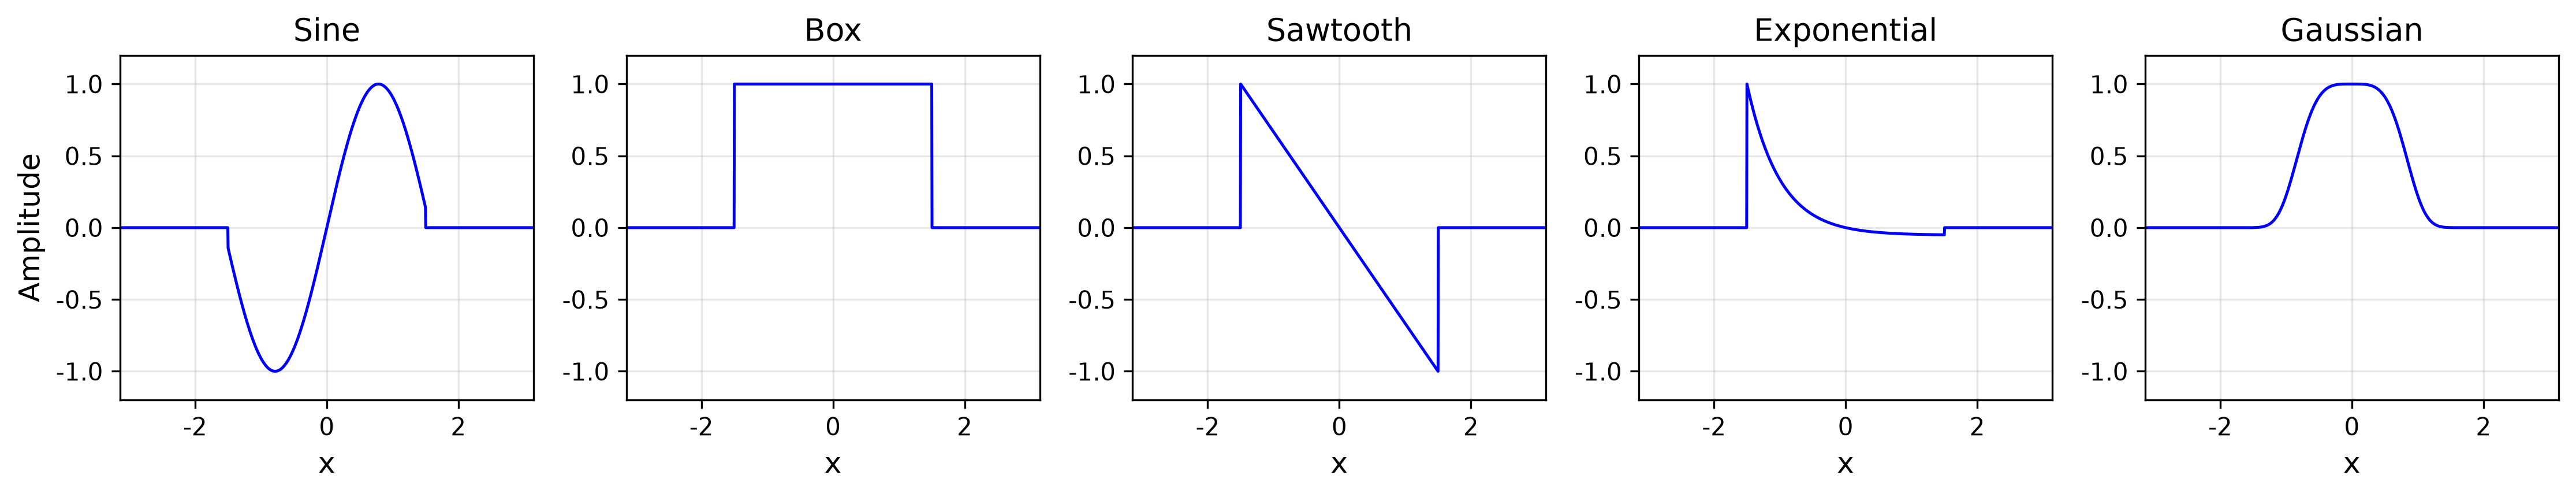
\includegraphics[width=0.8\textwidth]{../results/figures/fig1_signals.png}
	\caption{Pixel-Data Signals: Five distinct signal types (sine, box, sawtooth, exponential, and Gaussian) represented as discrete samples in the time domain.}
	\label{fig:signals}
\end{figure}

\begin{figure}[htbp]
	\centering
	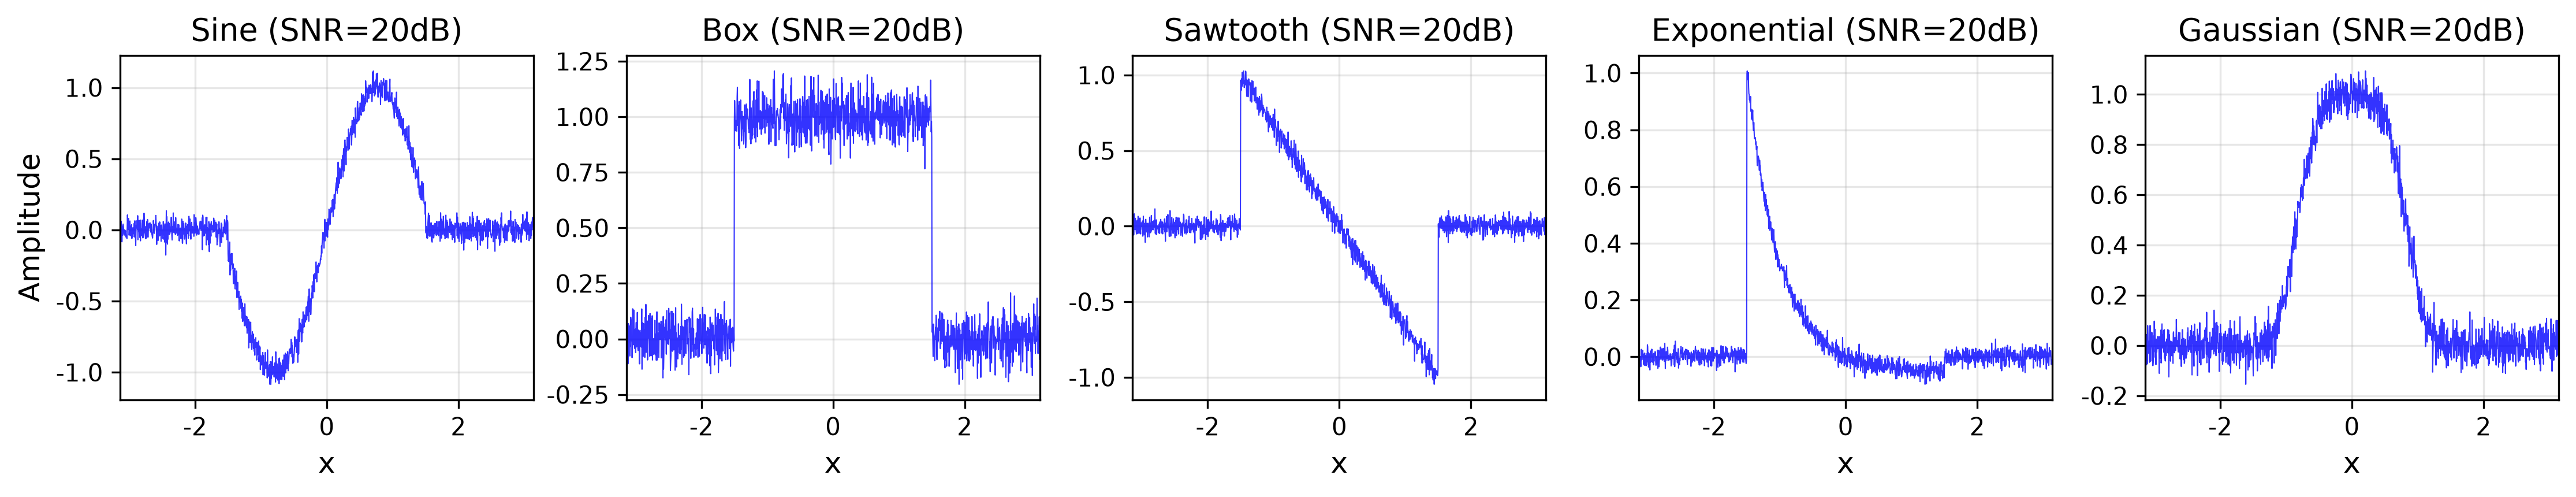
\includegraphics[width=0.8\textwidth]{../results/figures/fig2_signals_noise.png}
	\caption{Pixel-Data Signals corrupted with Gaussian noise (SNR = 20dB): The same five signal types with added noise to simulate real-world measurement conditions.}
	\label{fig:signalswnoise}
\end{figure}

\begin{figure}[htbp]
	\centering
	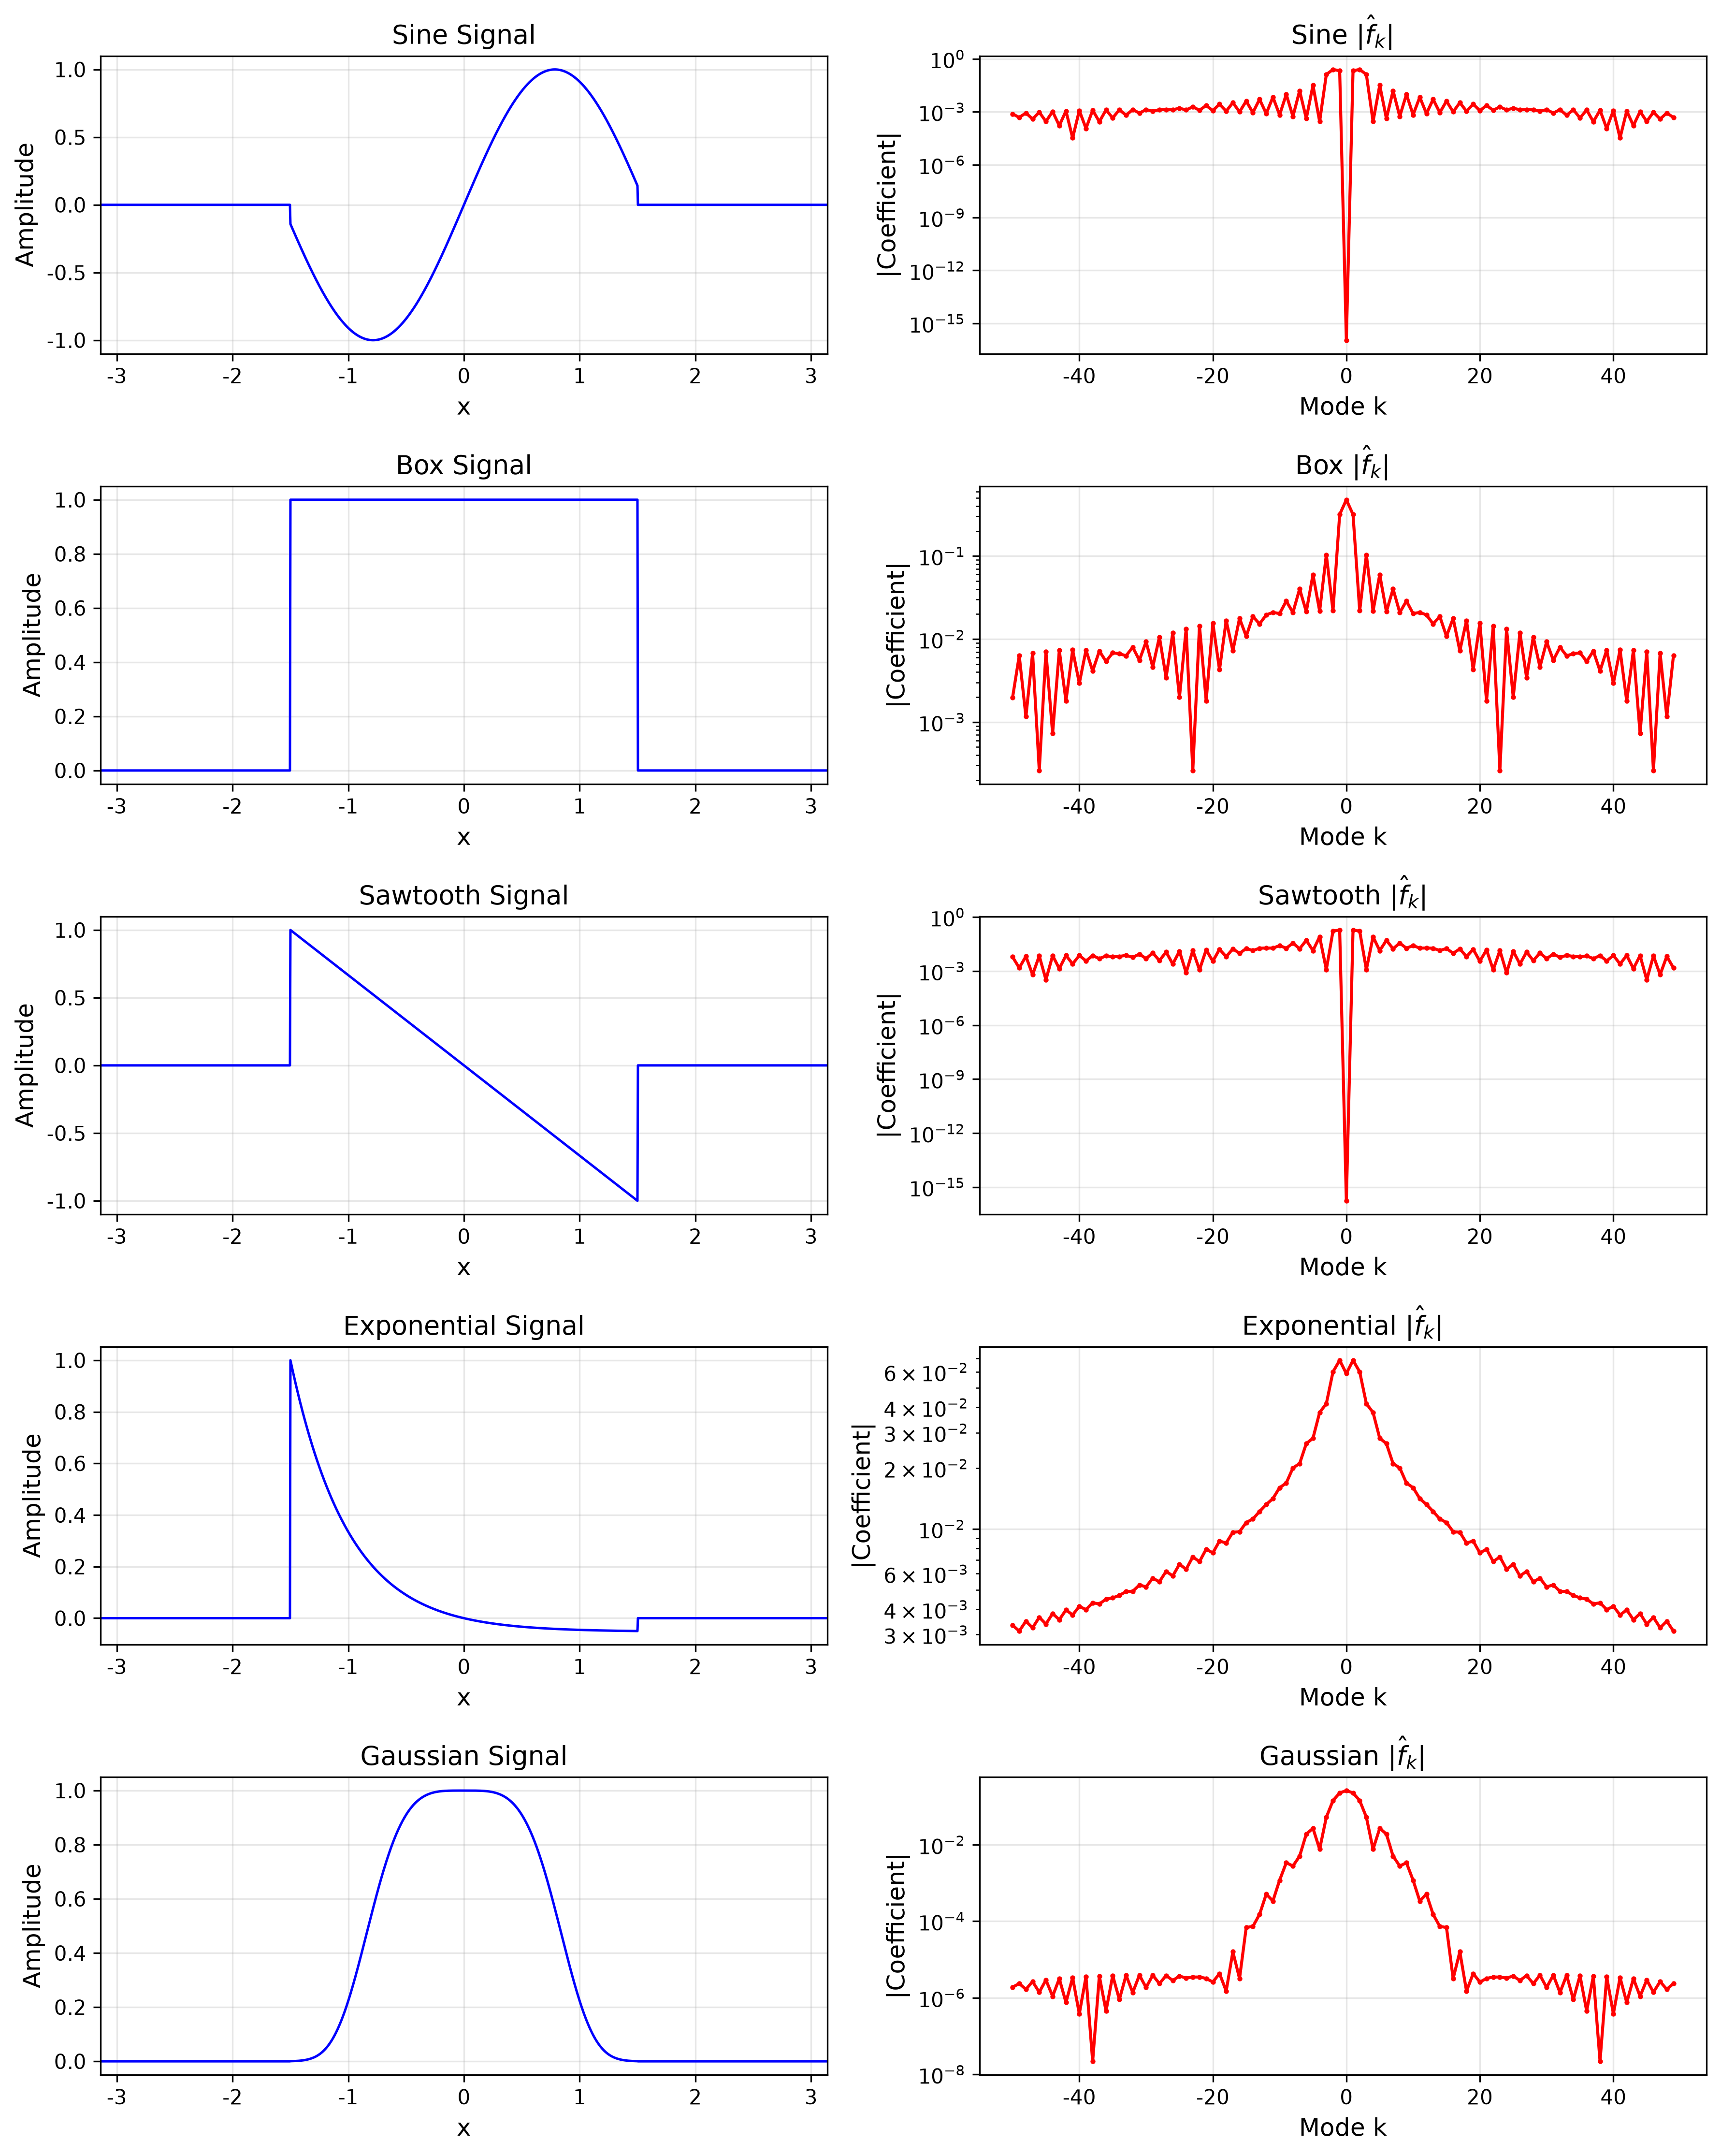
\includegraphics[width=0.9\textwidth]{../results/figures/fig3_signals_coeffs.png}
	\caption{Five different signal types (Sine, Box, Sawtooth, Exponential, and Gaussian) and their corresponding Fourier series coefficients. Each signal is normalized to have a maximum amplitude of 1. The Fourier coefficients show the frequency components present in each signal.}
	\label{fig:signals_and_coeffs}
\end{figure}

We implement our classifier using a feed-forward neural network, a standard machine learning algorithm. In typical signal classification tasks, neural networks are predominantly trained on grid-point data (i.e., discrete samples in the time domain). 
Therefore, we investigate the following questions:
\begin{enumerate}
    \item Does the performance of a classifier improve if it is instead trained using Fourier series approximations?
    \item How does the performance of a classifier depend on the number of terms (or equivalently, the number of Fourier series coefficients) used in such Fourier series approximations?
    \item Can the performance of such a classifier be improved by providing additional data, such as edges in the underlying (piecewise-smooth) signals?
\end{enumerate}

\section{Materials and Methods}
\subsection{Notations and Definitions}
\label{sec:defns} 

We use bold typeface and lowercase letters to denote vectors (for example, $\bx\in\C^{N}$) and capital letters in conventional typeface to denote matrices.

\begin{defn} ({\em Fourier Series, Coefficients and Partial Sum}) 
\label{defn:fourier_series_cfs} 
Let $f:\R\to\C$ be a $2\pi$-periodic function which belongs to the vector space $L^{2}(-\pi,\pi)$. We associate with $f$ the following series -- called the {\em Fourier series} -- 
\begin{equation}
	f\sim\sum_{k\in\Z}\widehat{f}_{k}e^{ikx},\label{eq:four_series}
\end{equation}
where the coefficients $\widehat{f}_{k}$ are defined as 
\begin{equation}
	\widehat{f}_{k}:=\frac{1}{2\pi}\int_{-\pi}^{\pi}f(x)e^{-ikx}dx,\qquad k\in\Z.\label{eq:four_cfs}
\end{equation}
Additionally, we define the $N$-th {\em partial Fourier sum} of $f$ to be 
\begin{equation}
	S_{N}f(x)=\sum_{|k|\leq N}\widehat{f}_{k}e^{ikx},\qquad x\in\R.\label{eq:partial_sum}
\end{equation}
\end{defn} 

\begin{defn} ({\em Jump Function, Locations and Values}) 
\label{defn:jump_fnc} 
Let $f:\R\to\C$ be a piecewise-smooth function. We define the {\em jump function} of $f$, denoted as $[f]$, to be 
\begin{equation}
	[f](x):=f(x^{+})-f(x^{-}),\quad x\in\R,\label{eq:jump_fnc}
\end{equation}
where $f(x^{+})$ and $f(x^{-})$ denote the right- and left-hand limits of $f$ at $x$ respectively. 
\end{defn} 

\subsection{Fourier Series and Discontinuities}

\subsubsection{Discrete Fourier Transform}
The Discrete Fourier Transform is used when the domain for $f$ consists of linearly spaced, discretized values. The Fast Fourier Transform (FFT) and its inverse (IFFT) are efficient algorithms that reduce the computational complexity from $O(n^2)$ to $O(n\log n)$ and are utilized for our purposes~\cite{osgood}.

\subsubsection{Accuracy of Fourier Approximations}
\label{subsec:accuracy}

The accuracy of Fourier approximations depends on the smoothness of the function being approximated. For smooth functions, Fourier series converge rapidly, while for functions with discontinuities, the convergence is slower and exhibits the Gibbs phenomenon near jump discontinuities.

\begin{figure}[htbp]
	\centering
	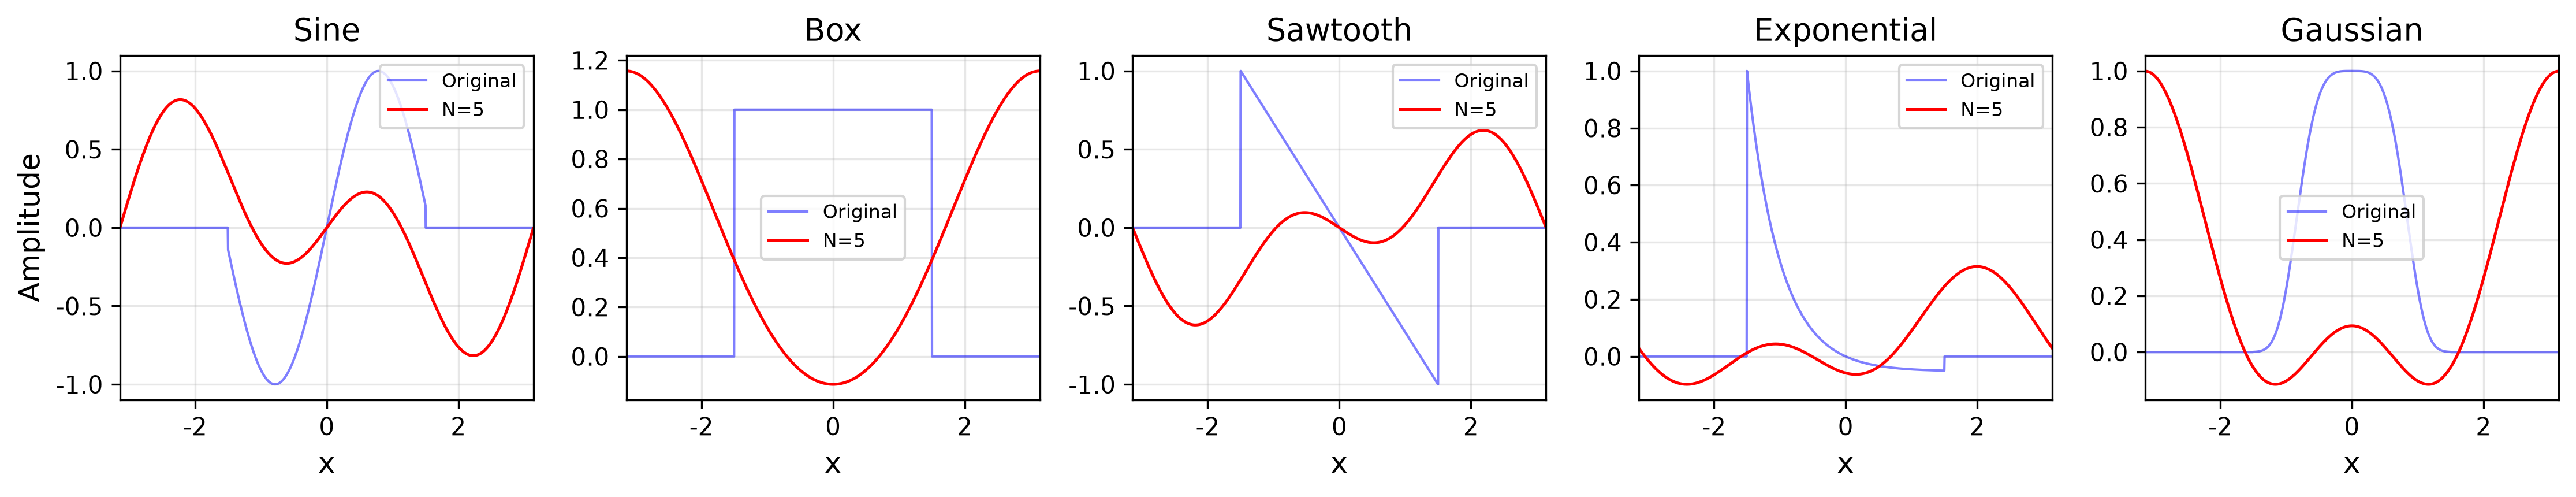
\includegraphics[width=0.8\textwidth]{../results/figures/fig_fourier_approx_N5.png}
	\caption{Low-frequency Fourier approximation (N = 5 modes): Note the poor approximation of discontinuities in the box and sawtooth signals.}
	\label{fig:fourierLow}
\end{figure}

\begin{figure}[htbp]
	\centering
	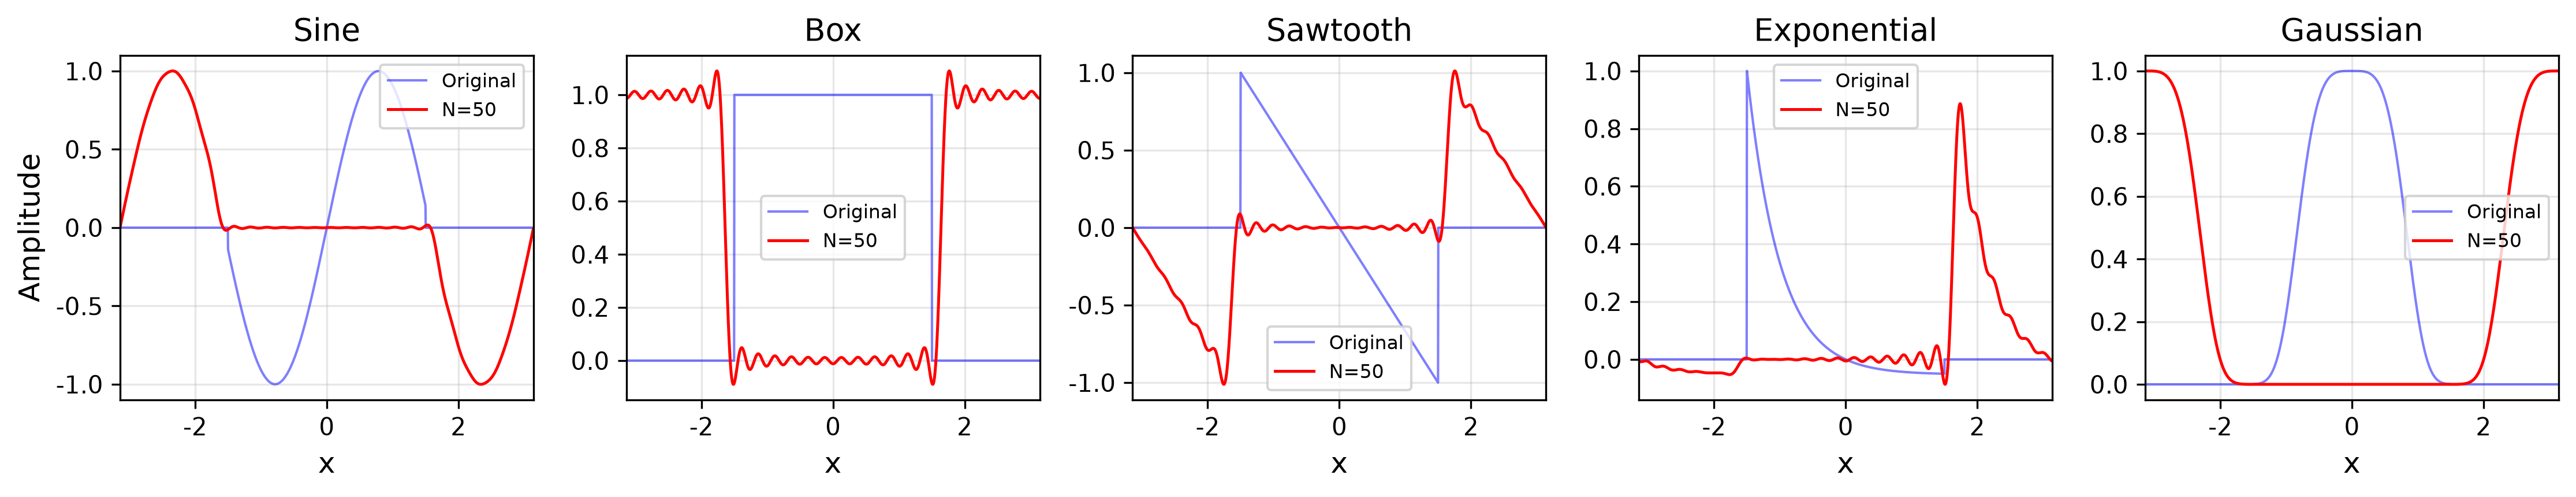
\includegraphics[width=0.8\textwidth]{../results/figures/fig_fourier_approx_N50.png}
	\caption{High-frequency Fourier approximation (N = 50 modes): Further improved approximation with reduced Gibbs phenomenon.}
	\label{fig:fourierHigh}
\end{figure}

\subsubsection{Obtaining Jump Data from Fourier Coefficients}
\label{subsec:jumpData}

Jump discontinuities in a function can be detected and quantified from its Fourier coefficients. For a function with jump discontinuities, the Fourier coefficients exhibit a slower decay rate ($|\hat{f}_k| \sim O(1/k)$) compared to smooth functions. 

To extract jump information, we use a procedure based on the work of Gelb and Tadmor~\cite{fourierCoef}, which leverages the non-linear enhancement of Fourier coefficients to identify discontinuities. The steps are as follows:
\begin{enumerate}
    \item Compute the Fourier coefficients $\hat{f}_k$ of the signal.
    \item Utilize the Generalized Conjugate Partial Fourier Sum, $S_N^g[f](x) = i \sum_{k=-N}^{N} \hat{f}(k) \text{sgn}(k) \sigma(\frac{|k|}{N}) e^{ikx}$, where $\sigma$ are known as concentration factors. Under these conditions, the concentration property $S_N^g[f](x) = [f](x) + O(\epsilon)$ holds, meaning the sum converges to the jump function at points of discontinuity.
    \item Extract both the locations and magnitudes of the jumps from the output of the concentration method. For the neural network input, the variable-length jump data is padded with zeros to a fixed maximum length.
\end{enumerate}

\begin{figure}[htbp]
	\centering
	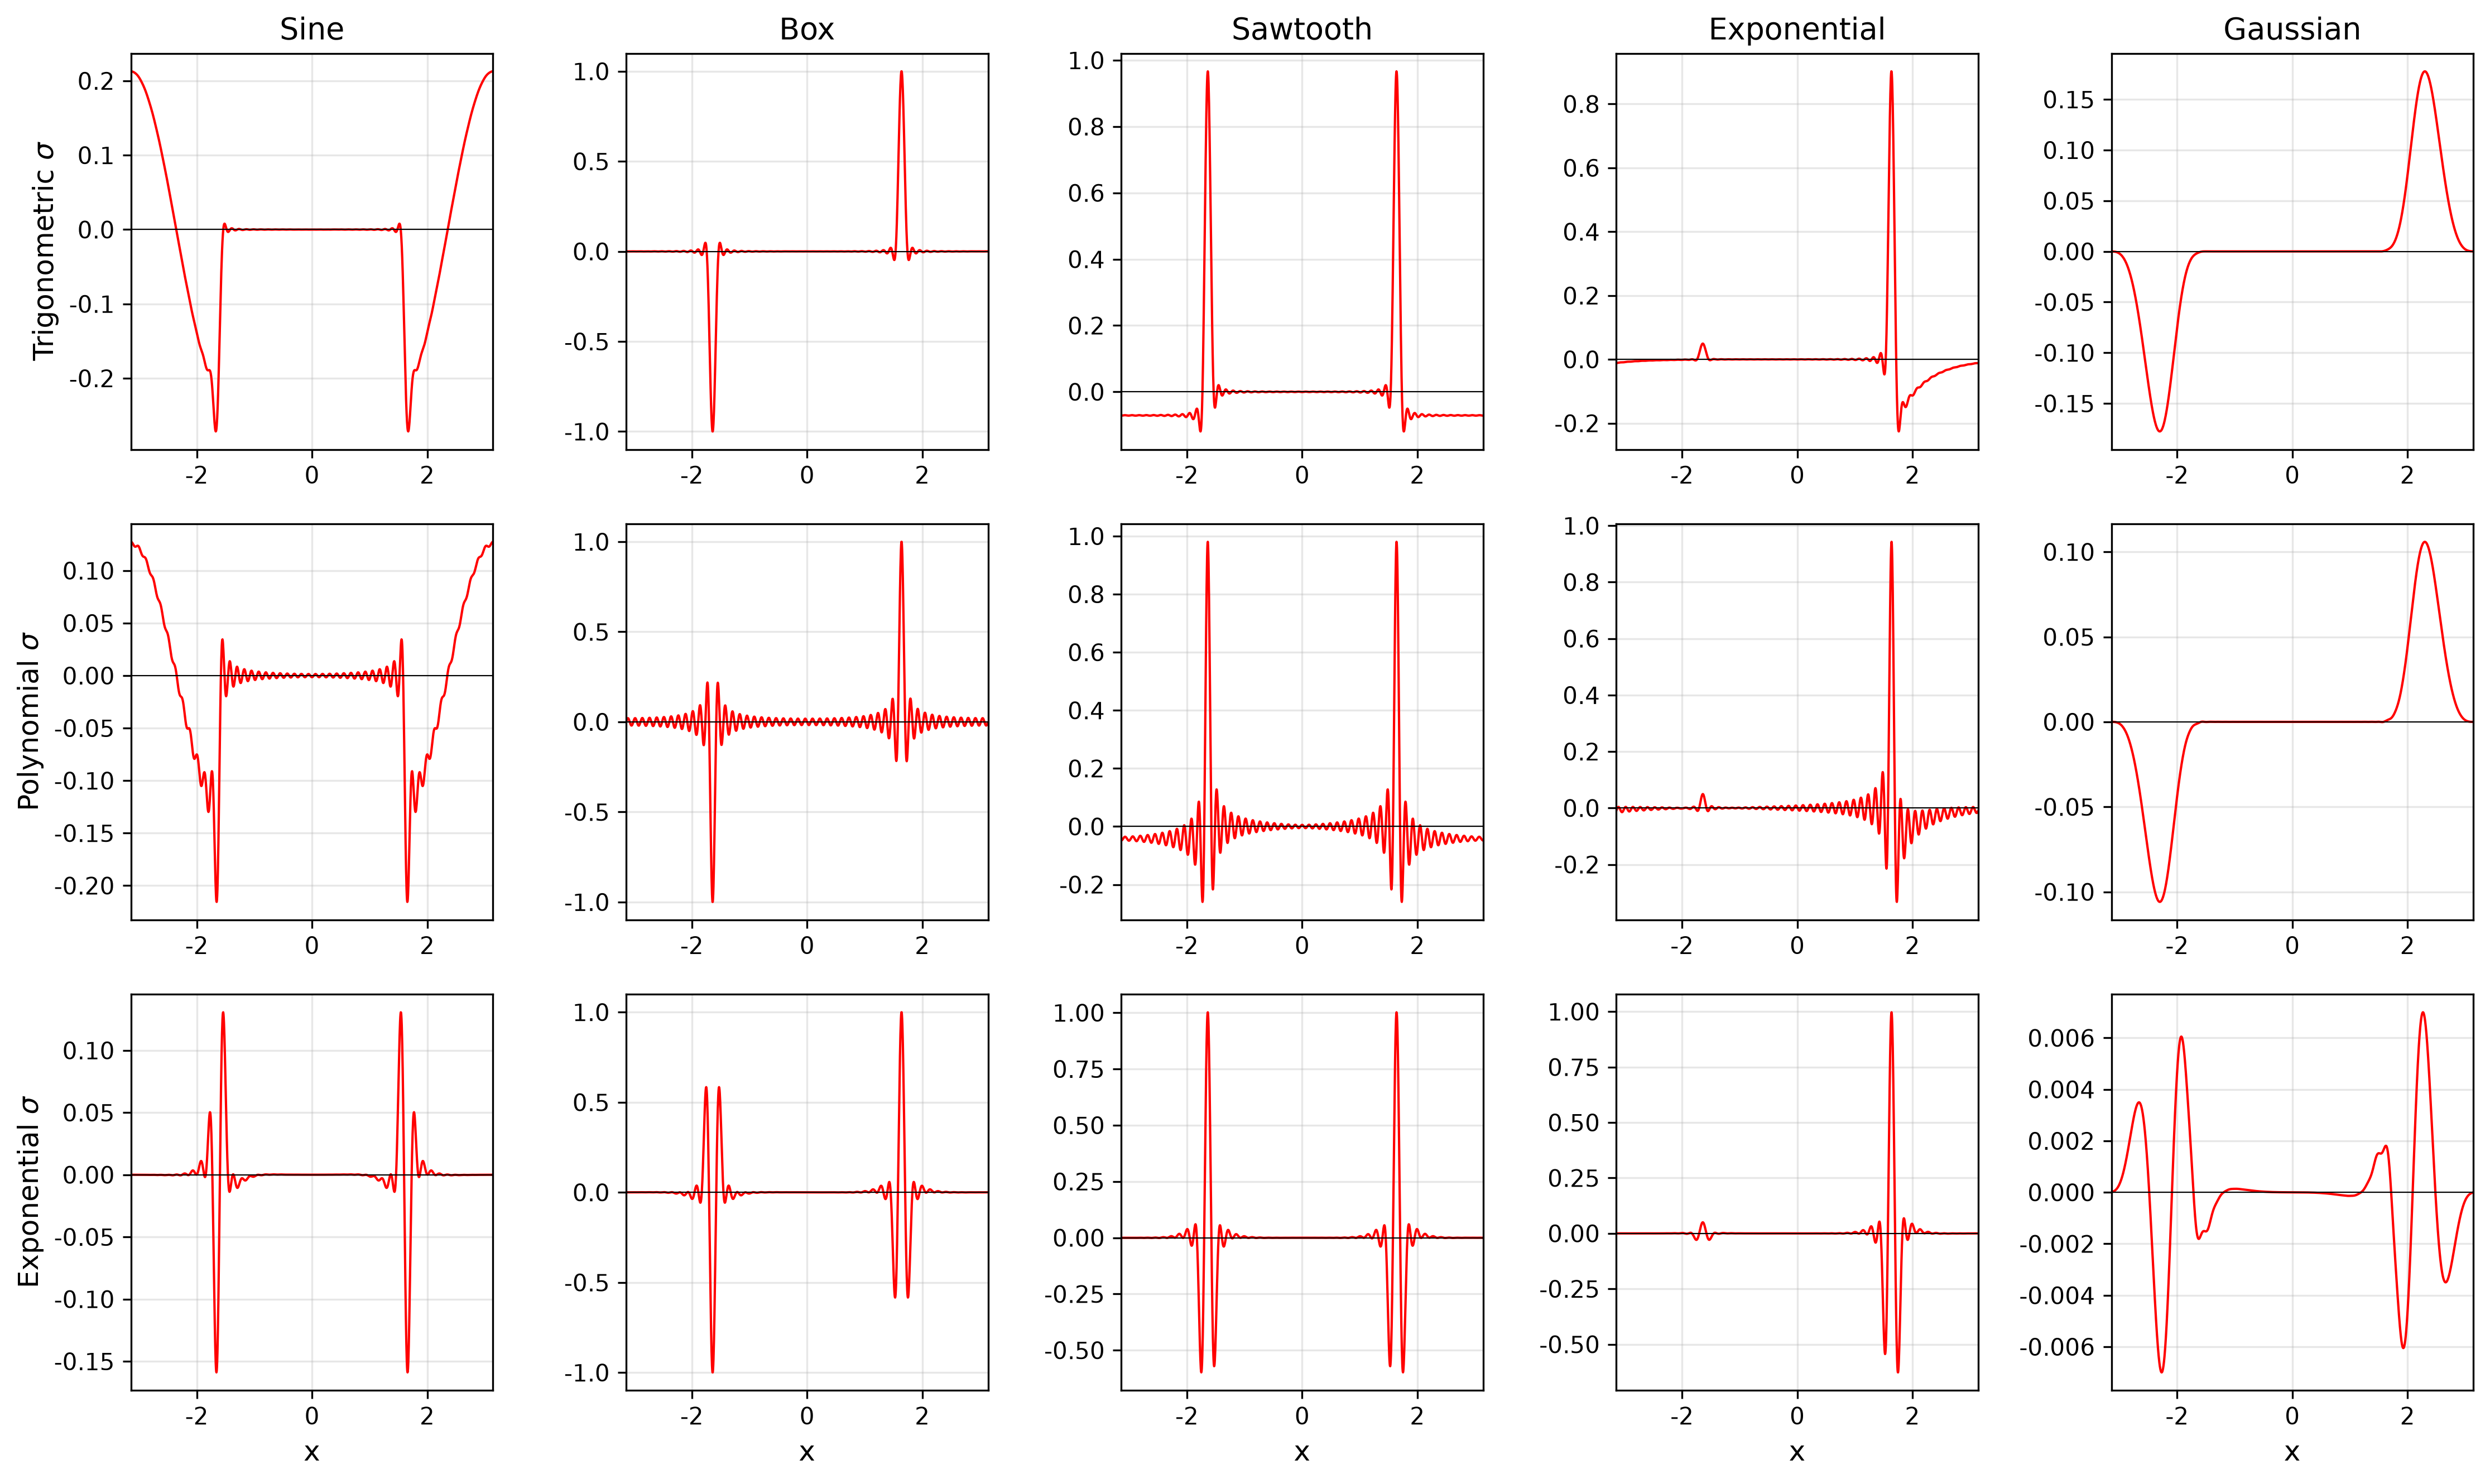
\includegraphics[width=0.9\textwidth]{../results/figures/fig7_edge_detection.png}
	\caption{Edge Detection using Concentration Factors: This figure illustrates the relationship between different signal types and the edge function computed using trigonometric, polynomial, and exponential concentration factors.}
	\label{fig:edge_detection}
\end{figure}

\section{Results}
\subsection{Signal Classification}
\label{sec:sig_Class}

We generated a dataset of five distinct signal types: sine, box, sawtooth, exponential, and Gaussian. Each signal was sampled at 1500 equally spaced points in the interval $[-\pi, \pi]$. The dataset was split into 70\% training, 10\% validation, and 20\% testing.

We trained three different neural network models:
\begin{itemize}
    \item \textbf{Model A}: Using raw signal data (1500 pixel values per signal).
    \item \textbf{Model B}: Using Fourier coefficients without jump information.
    \item \textbf{Model C}: Using Fourier coefficients with explicit jump information.
\end{itemize}

\subsection{Testing}
\label{subsec:testing}

\subsubsection{Model A}
Model A, trained on raw signal data, achieved an accuracy of 93.0\% on the clean test dataset. The model performed well on smooth signals but had difficulty distinguishing between signals with sharp transitions when noise was present.

\begin{figure}[htbp]
	\centering
	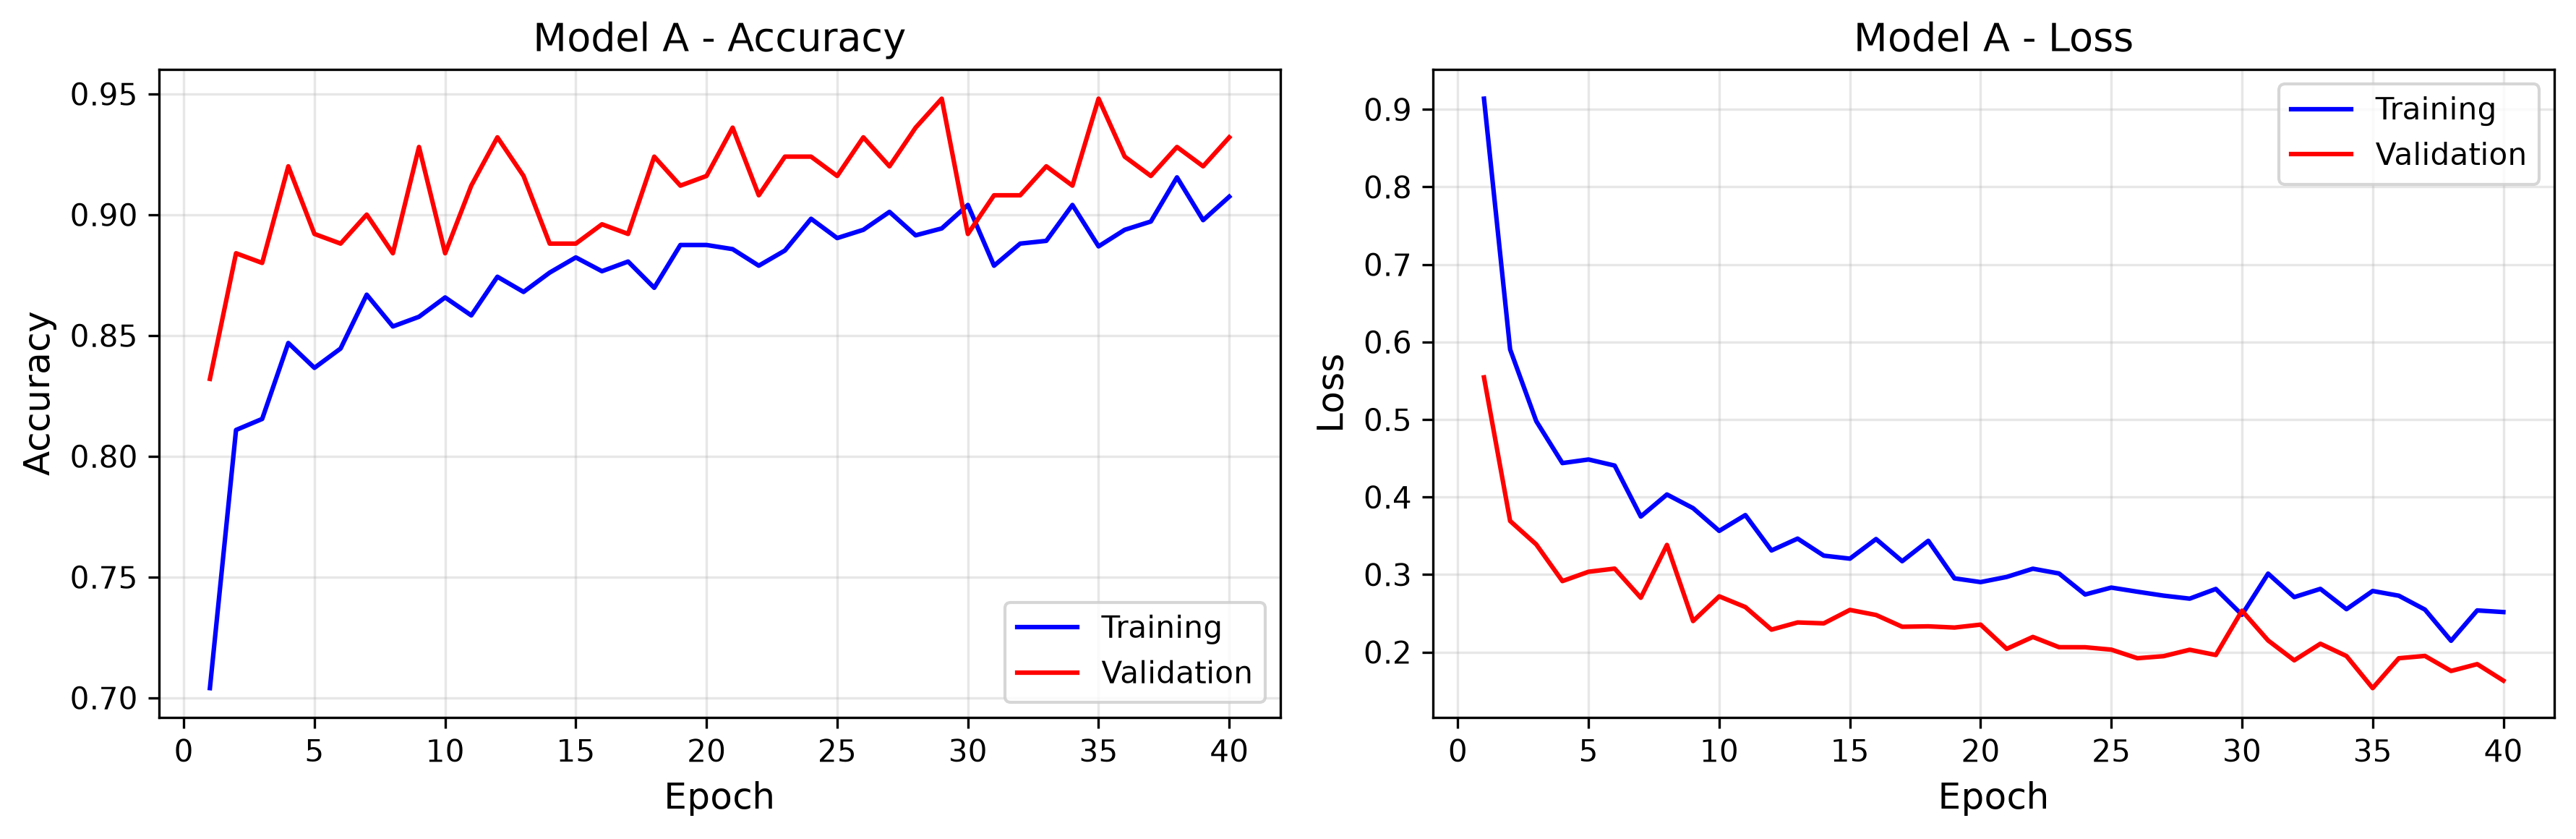
\includegraphics[width=0.8\textwidth]{../results/figures/fig_modelA_train.png}
	\caption{Model A training performance.}
	\label{fig:modelA1}
\end{figure}

\subsubsection{Model B}
Model B, trained on Fourier coefficients without jump information, achieved an accuracy of 93.2\% on the test dataset (with N=50 modes). Performance improves with more modes up to approximately N=50, after which diminishing returns are observed.

\begin{figure}[htbp]
	\centering
	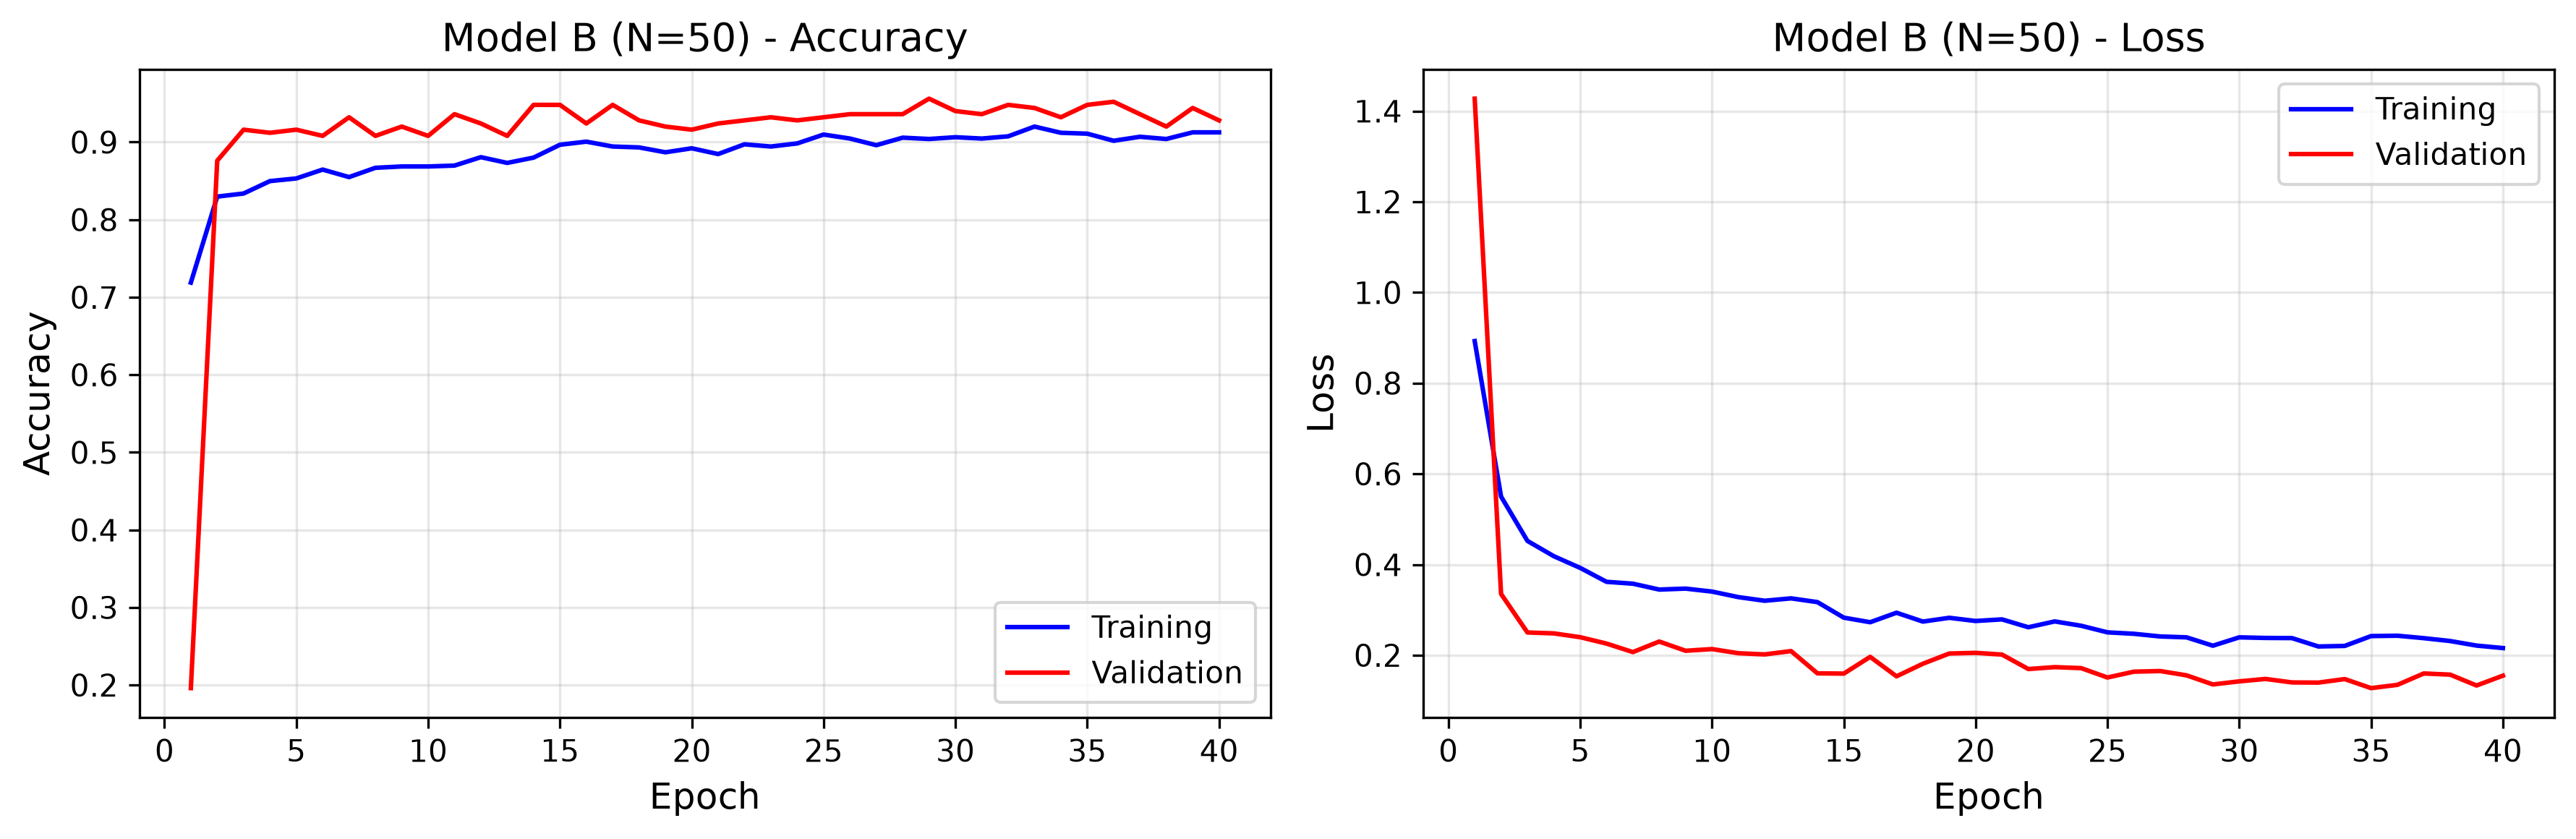
\includegraphics[width=0.8\textwidth]{../results/figures/fig_modelB_train.png}
	\caption{Model B training performance (N=50).}
	\label{fig:modelB1}
\end{figure}

\subsubsection{Model C}
Model C, trained on Fourier coefficients with explicit jump information, achieved an accuracy of 93.6\% on the test dataset (with N=50 modes). This model outperformed both Models A and B, particularly for signals with discontinuities.

\begin{figure}[htbp]
	\centering
	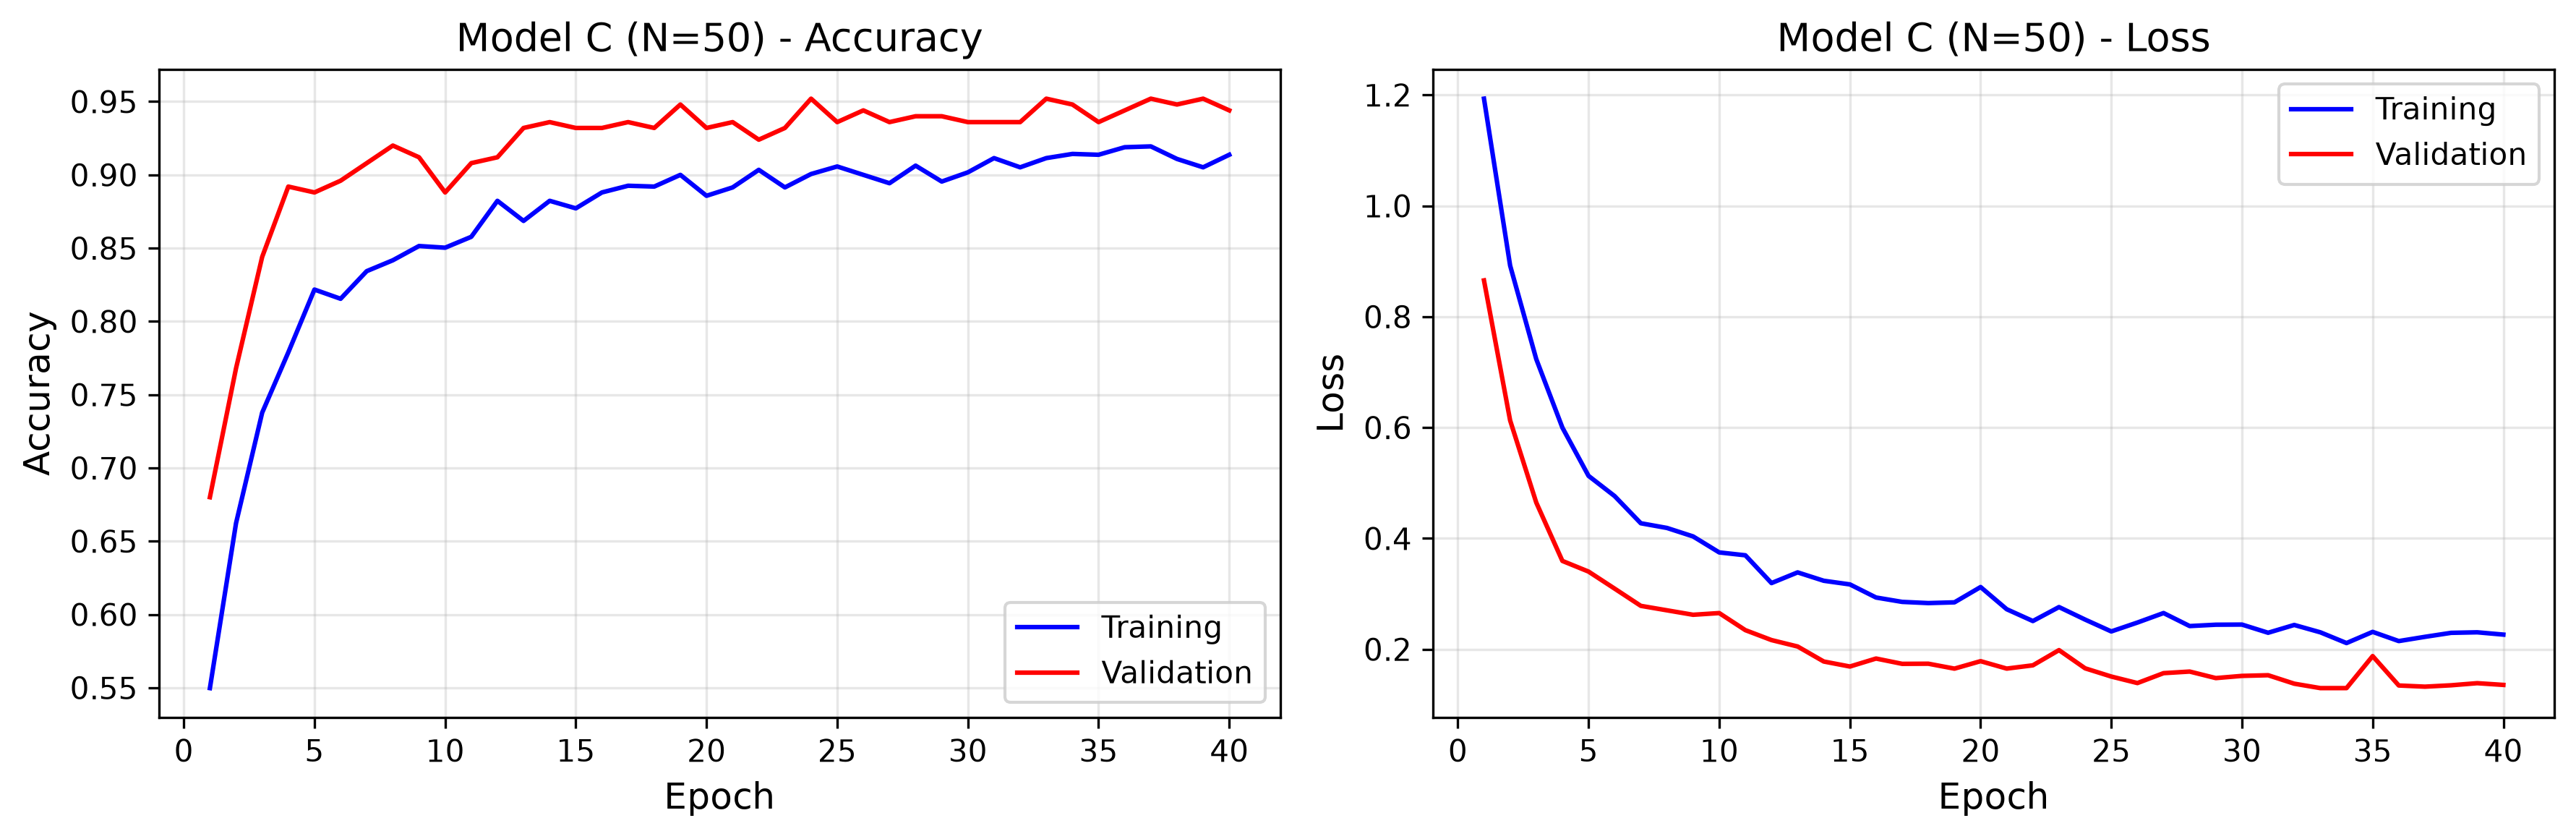
\includegraphics[width=0.8\textwidth]{../results/figures/fig_modelC_train.png}
	\caption{Model C training performance (N=50).}
	\label{fig:modelC1}
\end{figure}

\begin{figure}[htbp]
	\centering
	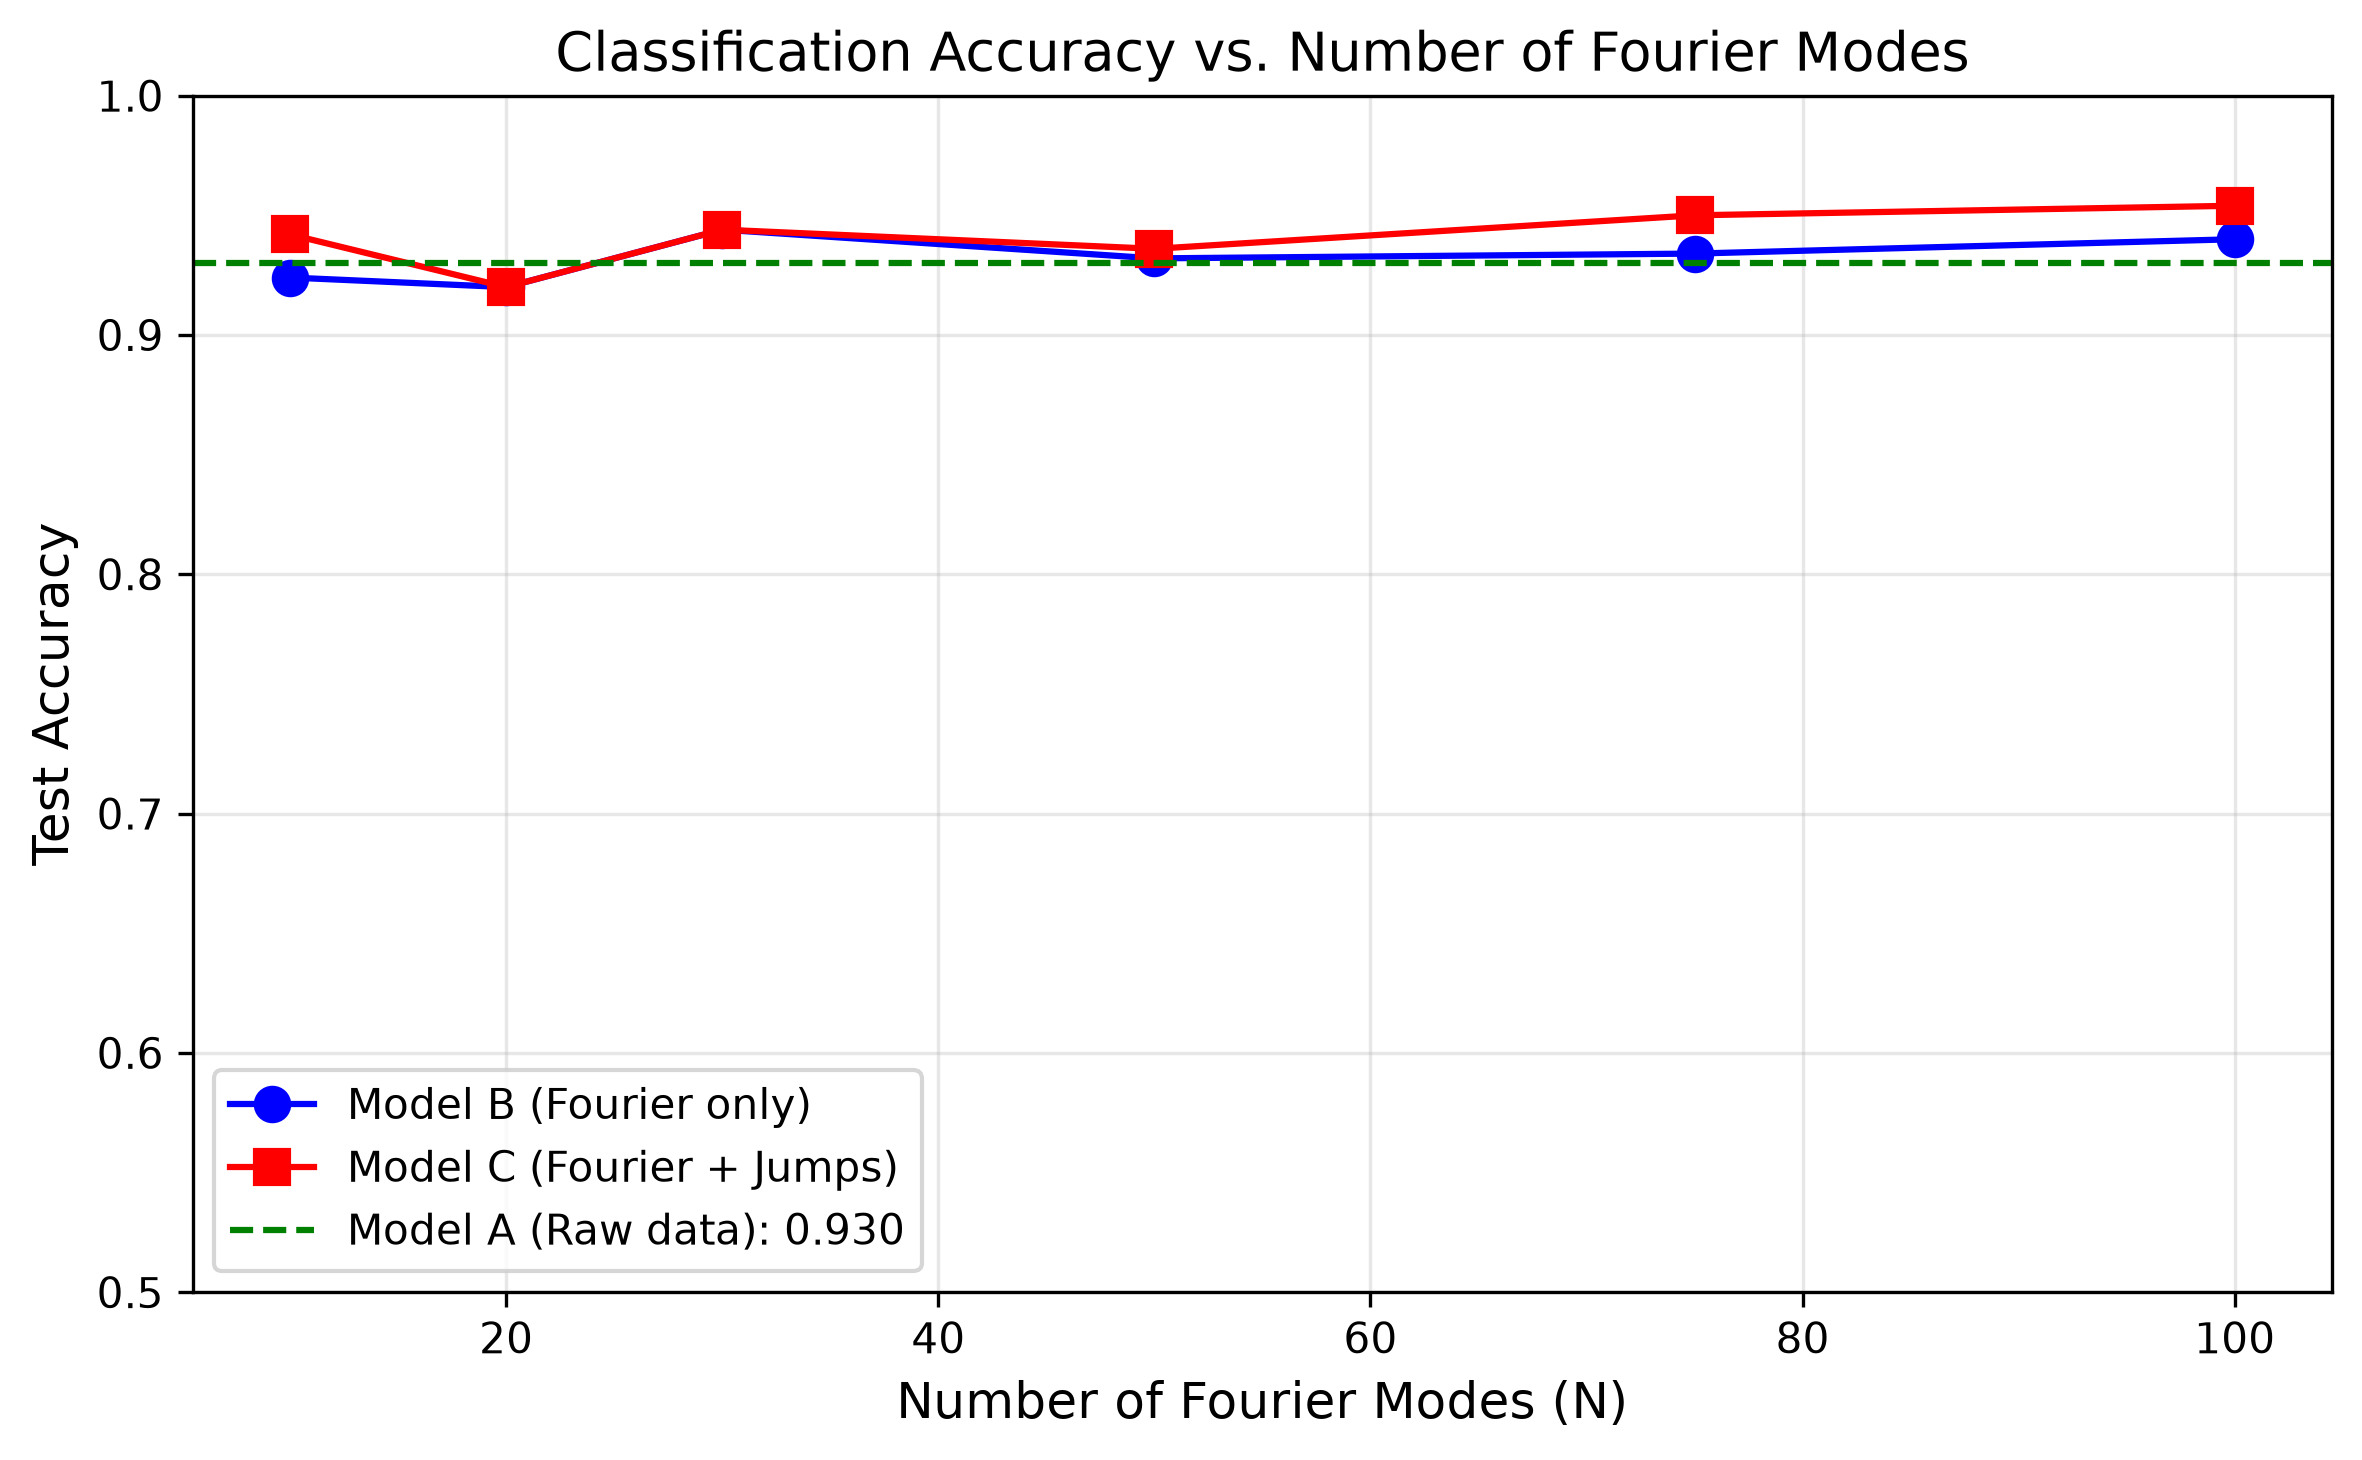
\includegraphics[width=0.8\textwidth]{../results/figures/fig_acc_vs_modes.png}
	\caption{Testing performance with varying numbers of Fourier modes: The graph shows classification accuracy as a function of the number of Fourier modes (N) used.}
	\label{fig:acc_vs_modes}
\end{figure}

\section{Discussion}

Our experimental results demonstrate that Fourier series coefficients can effectively replace grid-point data for neural network-based signal classification. Furthermore, the inclusion of jump information improves classification performance.

The performance of Model C (93.6\% accuracy) compared to Models A (93.0\%) and B (93.2\%) confirms our hypothesis that jump data contains critical information for signal classification. This finding aligns with the mathematical theory that discontinuities in signals are encoded in the asymptotic behavior of Fourier coefficients. The improvement from Model A to Model B suggests that the frequency domain representation itself provides advantages over the time domain representation, likely due to its ability to capture essential features with fewer dimensions. 

These findings have implications for signal processing applications where computational efficiency is important, as Fourier coefficients often provide a more compact representation than raw signal data.

\section{Conclusions}

This study investigated whether Fourier series coefficients can effectively replace grid-point data for neural network-based signal classification, and whether incorporating jump information improves classification performance. Our results provide strong evidence supporting both hypotheses.

The key findings of this research are:
\begin{enumerate}
    \item Fourier series coefficients can effectively replace grid-point data for signal classification, achieving comparable or better accuracy while reducing dimensionality.
    \item The inclusion of jump information enhances classification performance, with Model C achieving the highest accuracy.
    \item The number of Fourier modes used in the representation affects classification performance, with diminishing returns observed beyond approximately 50 modes for our dataset.
\end{enumerate}

These findings suggest that the mathematical properties of Fourier series can be leveraged in machine learning contexts to extract meaningful features that might otherwise be overlooked. 

\bibliographystyle{mdpi}
\bibliography{references}

\end{document}
